\documentclass{article}
\usepackage{enumitem}
\usepackage{fullpage}
\usepackage{fourier}
\usepackage{amsmath}
\usepackage{booktabs}
\usepackage{xspace}
\usepackage{hyperref}
\usepackage{graphicx}
\usepackage{color}
\usepackage[x11names]{xcolor}
\usepackage{multicol}
\usepackage{wrapfig}

\newcommand{\red}[1]{\textcolor{red}{#1}}

\usepackage{fancyhdr}
\pagestyle{fancy}
\fancyhf{}

\fancypagestyle{plain}{%
  \fancyhf{}
  \renewcommand{\headrulewidth}{0pt}
  \renewcommand{\footrulewidth}{0pt}
  \lfoot{\textcopyright{} 2021 Darrell Long}
  \rfoot{\thepage}
}

\pagestyle{plain}


\title{CSE 13S: Computer Systems and \textbf{C} Programming}
\author{Prof.\xspace Darrell Long}
\date{Spring 2021}

\begin{document}\maketitle
\begin{quotation}
\emph{
C programming, command line, shell programming, editors, debuggers,
source code control, and other tools. Basic computer systems,
algorithm design and development, data types, program structures.
Develops understanding of process model, compile-link-execute build
cycle, language-machine interface, memory, and data representation.
Students cannot receive credit for both CSE 13S and CSE 13E. Course
is $7$ units $(5 + 2)$ with integrated laboratory.
}
\end{quotation}

\section{Introduction}

For this course, you are expected to have some programming experience.
This experience usually takes the form of assembly language in CSE
12/L, and you may also have taken CSE 20 or CSE 30, and so may have
some experience programming in Python. Please be aware that programming
in \textbf{C} is more like programming in assembly language than
in Python: you are exposed to the machine, and it will not try to
prevent you from making mistakes.

You are expected to have a certain level of mathematical maturity,
corresponding approximately to Algebra 2, although it would be best
if you had just a little Calculus since we will use derivatives in
the lecture.

You will learn the rudiments of some fundamental data structures:
arrays, pointers, bit vectors, stacks, queues, hash tables, and
simple trees. You will learn how to create abstract data types in
a language that does not support object-orientation. You will learn
about dynamic memory management and how to twiddle bits.

You will be learning to use many tools that are common to \textsc{Unix}
(and have been ported to other operating systems as well). There
are more tools than we can cover during the quarter, so you are
expected to learn how to find the right tool for the job. You are
encouraged to share with your fellows the tools that you find---but
not the code that you write to use them.

You will encounter debuggers, static, and dynamic code analyzers.
You will see how code is translated from \textbf{C} to assembly
language to machine code and then executed as a process.

You will learn computer systems concepts such as processes, memory,
files, permissions, and the like. Ideally, at the end of this course,
you will be comfortable operating in a \textsc{Unix} environment.

\textcolor{red}{Some of you will resist using \textsc{Unix}. This
intransigence is a mistake of epic proportions that you will regret
when you move on to other courses. Learn it now while you have
support.}

\section{Reading}

One of the most important lessons during your time in college is
\emph{learning how to learn on your own}. To a certain extent, that
means that you need to learn to be an autodidact. You do this by
reading; reading books, manuals, and published articles. These are
not skills that you can learn by only watching videos on the Internet.

\subsection{Required}

All of your professors learned to program in \textbf{C} using the
classic text by Kernighan \& Ritchie.  Here in the United States
the cost is \$59 on \url{Amazon.com}, but it is only \$3.73 on
\url{Amazon.in} (the last time I checked).  Take from that what you
will regarding the pricing policies of the publishers.

\begin{itemize}
\item
Brian W. Kernighan and Dennis M. Ritchie. \emph{The C Programming Language}. 2006.
\end{itemize}

It is important for you to understand that \textcolor{red}{reading}
\emph{The C Programming Language} is not a suggestion, it is a requirement. You must
read it. And to then to read it again.  This is not a onerous
task: the book is not long, you can read it in an afternoon. That
is the beauty of this book, and of the \textbf{C} language.

\textcolor{red}{Many of you will refuse to read the book; this is as large of a mistake as not
learning \textsc{Unix}. You will regret it, and you will be asked when you come to office hours:
``Did you read the book?'' If the answer is ``no'' then you will be sent to the end of the queue.}
\subsection{Recommended}
On the campus network, access to many electronic books is \emph{free of
charge}. This is an enormous boon to you, and you are strongly encouraged to
take advantage of it.

If you follow this link:
\url{https://proquest-safaribooksonline-com.oca.ucsc.edu }
you will find \emph{many} electronic books that will be useful in
this course (and others). We will suggest some readings in these
books: please, do not ignore those suggestions.

Here are some of the books that we will refer to during the course of the
quarter:
\begin{itemize}
  \item J.\xspace Loeliger \& M.\xspace McCullough. \emph{Version Control with
    Git}.
  \item C.\xspace Newham \& B.\xspace Rosenblatt. \emph{Learning the bash
    Shell}.
  \item A.\ Robbins, E.\ Lamb \& L.\ Hannah, \emph{Learning the vi and Vim
    Editors}.
  \item A.\ Robbins, E.\ Siever, S.\ Figgins \& R.\ Love. \emph{Linux in a
    Nutshell}.
  \item T.\ Crawford \& P.\ Prinz. \emph{C in a Nutshell}.
  \item R.\ Mecklenburg. \emph{Managing Projects with GNU Make}.
  \item W.\ Shotts. \emph{The Linux Command Line}.
  \item G.\ Neville-Neil. \emph{The Kollected Kode Vicious}
\end{itemize}

\section{Grading}
In this course, you will have a final examination that counts for 30\% of your
grade. The final examination is comprehensive, and you can expect it to cover
all of the material that you have learned in the course. You will be allowed
to bring \textcolor{red}{one sheet of notes} to the examination. Electronics
of any kind, excluding medical devices, are disallowed.

\textcolor{red}{This quarter we will be virtual using Zoom, so it will not be possible to enforce
this restriction but we ask that you honor this request.}

We will have weekly quizzes this term. The quizzes will be
opened on Friday, closed on Saturday. You will have 60 minutes to complete them.
It should go without saying---but obviously it does not---that you must
complete these quizzes on your own, with no help from any other person
(including virtual persons on the Internet).

\textcolor{red}{We will use all tools available to us, including
Canvas, to verify that you are not using Google to find the answers.}

These quizzes are in replacement of a midterm examination and count
for 20\% of your grade. This saves us from losing a day to the
midterm.
\textcolor{red}{Do not forget to take the quiz! There is no making up of missed
quizzes.}

The programming assignments are worth 50\% of your grade. You are strongly
encouraged to attend the laboratory sections where specifics of each
assignment will be discussed. But do not expect the TA or the tutors to write
your code for you: they can help you to find bugs, and offer suggestions, but
the ideas in the code must come from you, and the typing of the code must be
done by you.

The points are allocated to assignments based on difficulty. For example,
assignment 0, which is trivial, has very few points allocated to it. The
assignment where you implement several sorting algorithms and do some
comparison and analysis has correspondingly more points associated with it.

\textcolor{red}{Remember: We will release assignments one week early. We are
doing this in hopes of encouraging you to start early. It would be a mistake to
not take advantage of this policy.}

\section{Laboratory Exercises}

Since many of you will be reluctant to learn \textsc{Unix}, we will have weekly
mandatory laboratory exercises presented by each of the TAs in section. This
section is \emph{in addition} to the section were programming assignments are
discussed.

\textcolor{red}{Skip these sections at your own peril!} We will be describing
\textsc{Unix} tools that you will need in order to complete assignments.

\section{Programming}
The most important component of this course will be programming in the
\textbf{C} programming language. You will also learn to program using
\texttt{make}, \texttt{bash}, and many other tools.

The programs start out trivial---a junior-level student should be able to
complete the first assignment in about 10 minutes---but rapidly increase in
difficulty. The first six assignments are allocated one week; the last two
assignments are allocated approximately two weeks each.

Here is a list of the programming assignments for the quarter:
\begin{multicols}{2}
\begin{enumerate}[start=0]
  \item ``Hello World!''
  \item Simple Game
  \item Simple numerical library
  \item Shortest path finding
  \item Game of Life
  \item Sorting
  \item Hashing \& Linked Lists
  \item Data Compression
\end{enumerate}
\end{multicols}

You will be using a lot of tools, some which you may have never seen before. You
will, for example, be using the \emph{command line}:
\begin{quotation}
\centerline{\url{http://www.linuxcommand.org/tlcl.php}.}
\end{quotation}
You may think---but you would be incorrect---that the command line is out-dated,
less powerful, or some other misconception. In reality, the command line is the
most powerful since it is a language in which you can express programs about
programs. Often, the Graphical User Interface (GUI), is simply a wrapper around
commands for the command line. \textcolor{red}{Once again, it would be a
mistake for you to try to avoid the command line in this course.}

We will release the assignments at least a week early, effectively giving you up
to an extra week if you complete the previous assignment before it was due. You
are strongly encouraged to take advantage of this practice and start your
assignments as early as you understand the material necessary to do so.

\textcolor{red}{One of the great mysteries of the universe is that many of you
will start the assignment a day or two before it is due. This too is a mistake.
More mysterious, is that a number of you will persist in this error through all
of the assignments, losing points unnecessarily.}

\textcolor{red}{Remember: You are required to submit the \texttt{git} commit ID
you want graded for each assignment on Canvas. Failure to submit a commit ID
means no grade for that assignment.}

\subsection{Late Policy}
The late policy is simple: you lose 25\% per day, for the first 3 days, after
that you will receive a \emph{zero}. If you turn your assignment in on-time,
then you are eligible to receive full points. One day late, you can earn at most
75\% of the available points; two days late, you can earn at most 50\%. This
continues until the third day, when you are no longer eligible for any points.

\centerline{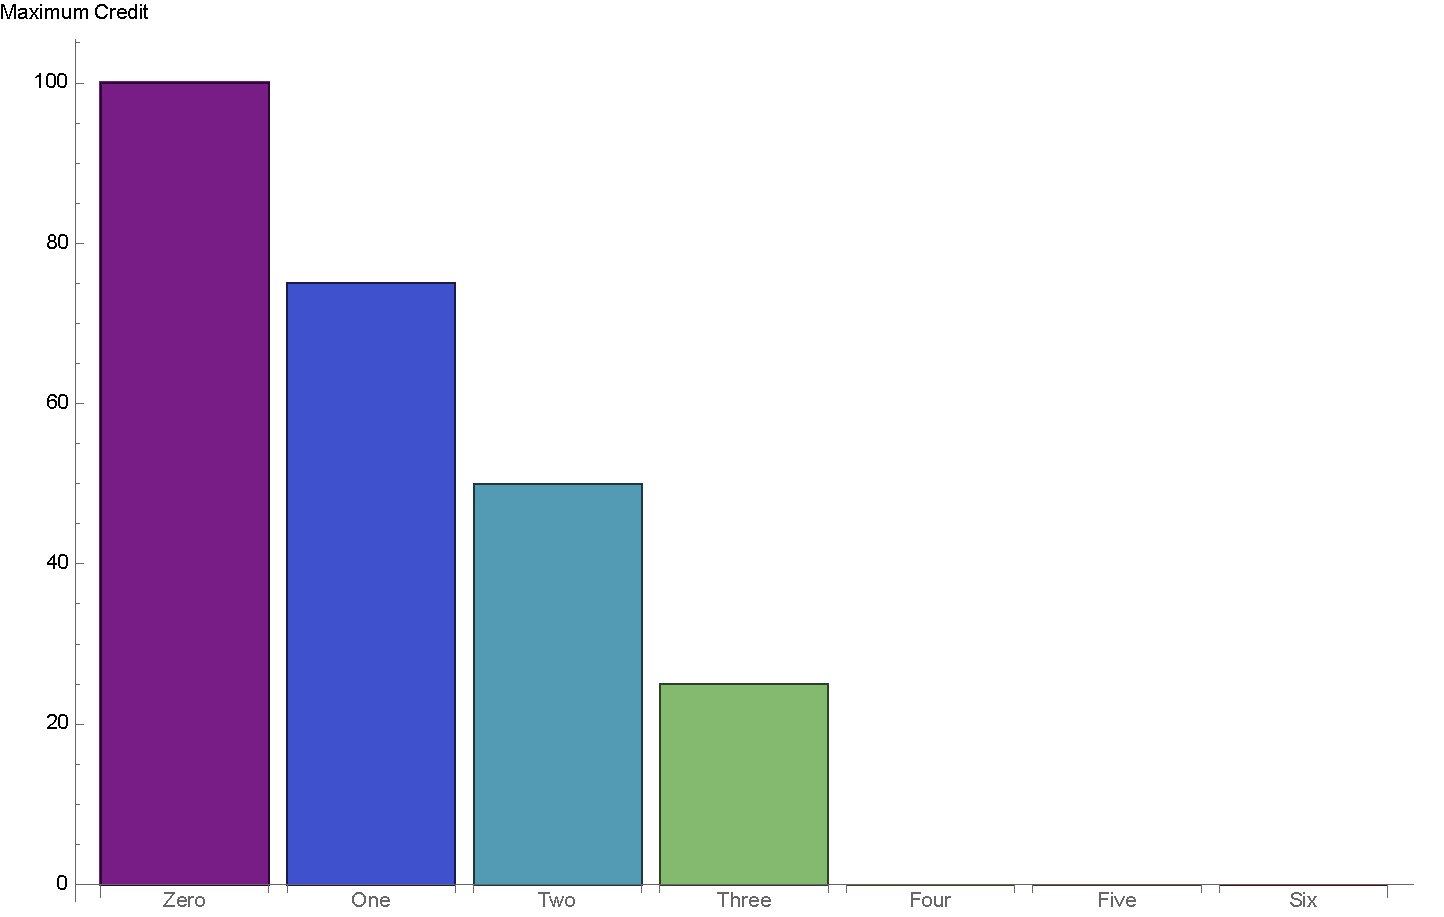
\includegraphics[width=0.75\textwidth]{Tardiness.pdf}}

If you have a medical emergency, please provide a note from the attending
medical professional. If you have a family emergency, please discuss it with me.
Depending on the nature of the emergency, documentation may be required. If your
computer is lost, stolen, or broken, you can take comfort that since you used
\texttt{git} correctly you did not lose any of your work.

\section{Schedule}

The schedule of suggested readings and assignments will be posted on Canvas and
kept up to date. You will also find the quizzes there each Friday.

\section{Academic Honesty}

The unfortunate reality is that academic dishonesty occurs frequently, and most
of the time it happens in introductory courses. Consequently, you will be
reading and signing (via \texttt{git} submission) a statement regarding this
topic. \emph{Your assignments will not be graded until you have done so.}

Academic dishonesty of any kind is forbidden. If you conduct yourself as a
person of integrity you will have no problems.

You are expected to adhere to the highest standards of academic
integrity.
This means that plagiarism\footnote{{\bf pla$\cdot$gia$\cdot$rize} {\em vt.}
[$<$ L. {\em plagiarius,} kidnaper] to steal and pass off as one's own
(the ideas or words of another) to present as one's own an idea or product
derived from an existing source -- {\bf pla$\cdot$gia$\cdot$riz$\cdot$er}
{\em n.} (source: Webster's New World Dictionary)}
in any form is unacceptable.
As a (soon to be) computing
professional, you are encouraged to consult the code of ethics
appropriate to your discipline.\footnote{The Association for Computing Machinery
is \url{http://www.acm.org/}, the IEEE is
\url{http://www.ieee.org/} and the IEEE Computer
Society is \url{http://www.computer.org/}.}

All work submitted that bears your name must be exclusively your own.
The copying or providing to other students, in whole or in part,
solutions (text or source code) to class assignments from any source
(including work done by former or current Computer Science \& Engineering students,
other humans, animals, zombies, sparkling vampires, the Bavarian Illuminati,
any of the Four Horsemen of the Apocalypse, or materials found
on the Internet, \emph{et cetera}) that are not explicitly sanctioned by me or
the teaching assistants is unacceptable.

All material that did not originate with you must be \emph{cited}
-- you must credit the source in all cases. You will not get credit
for this work, but this is \emph{not considered cheating}. Information and
assistance from the professor, teaching assistants, assigned project partners (if applicable),
course textbooks, course web site, and code and documentation
(\emph{e.g.}, \texttt{man} pages) supplied with the \textbf{C} Standard Library
(\texttt{libc}) may be freely used without acknowledgment.

There is no flexibility in this policy. If you cheat, you fail, and
your academic career may be prematurely foreshortened. The
\emph{reason} that you cheated is entirely immaterial. This policy
applies equally to all parties, regardless of whether they are
transmitting or receiving the material in question. A more exhaustive description
of the consequences and process for academic misconduct
appear in the university's policy on academic honesty which is listed at:
\url{https://ue.ucsc.edu/academic-misconduct.html}.

\section{DRC Accommodations}
DRC accomodations must be reasonable, and must specify what you
need. You must also tell us in advance. If you have, for example,
$1.5\times$ time on examinations it does not transfer to programming
assignments. In general, we can give you \emph{one extra day}, but
you cannot tell us the day it is due. If you are having a ``flare
up'' then you need to let us know so we can make adjustments.
\textcolor{red}{\emph{There are no late days on the final assignment.}}

We are committed to creating an academic environment that
supports its diverse student body. If you are a student with a
disability who requires accommodations to achieve equal access in
this course, please submit your Accommodation Authorization Letter
from the Disability Resource Center (DRC) to me privately during
my office hours or by appointment, preferably within the first two
weeks of the quarter. At that time, I would also like us to discuss
ways we can ensure your full participation in the course. I encourage
all students who may benefit from learning more about DRC services
to contact DRC by phone at (831) 459-2089 or \url{drc@ucsc.edu}.

\section{Title IX and CARE}
We are committed to providing a safe learning environment
that is free of all forms of gender discrimination and sexual
harassment, which are explicitly prohibited under Title IX. If you
have experienced any form of sexual harassment, sexual assault,
domestic violence, dating violence, or stalking, know that you are
not alone. The Title IX Office, the Campus Advocacy, Resources and
Education (CARE) office, and Counseling and Psychological Services
(CAPS) are all resources that you can rely on for support.

Please be aware that if you tell me about a situation involving Title IX
misconduct, I am required to share this information with the Title IX
Coordinator. This reporting responsibility also applies to course TAs and tutors
(as well to all UCSC employees who are not designated as ``confidential''
employees, which is a special designation granted to counselors and CARE
advocates). Although I have to make that notification, you will control how your
case will be handled, including whether or not you wish to pursue a formal
complaint. The goal is to make sure that you are aware of the range of options
available to you and that you have access to the resources you need.
Confidential resources are available through CARE. Confidentiality means CARE
advocates will not share any information with Title IX, the police, parents, or
anyone else without explicit permission.  CARE advocates are trained to support
you in understanding your rights and options, accessing health and counseling
services, providing academic and housing accommodations, helping with legal
protective orders, and more. You can contact CARE at (831) 502-2273 or
\url{care@ucsc.edu}.

\end{document}
